\documentclass[11pt,a4paper]{article}

% These are extra packages that you might need for writing the equations:
\usepackage{amsmath}
\usepackage{amsfonts}
\usepackage{amssymb}
\usepackage{booktabs}
\usepackage{hyperref}
\usepackage{listings}
\usepackage{xcolor}
\lstset {language=C++,
		 basicstyle=\ttfamily,
         keywordstyle=\color{blue}\ttfamily,
         stringstyle=\color{red}\ttfamily,
         commentstyle=\color{purple}\ttfamily,
         morecomment=[l][\color{magenta}]{\#},
       	 basicstyle=\tiny}

% You need the following package in order to include figures in your report:
\usepackage{graphicx}

% With this package you can set the size of the margins manually:
\usepackage[left=2cm,right=2cm,top=2cm,bottom=2cm]{geometry}


\begin{document}

% Enter the exercise number, your name and date here:
\noindent\parbox{\linewidth}{
 \parbox{.25\linewidth}{ \large HPCSE I, Exercise 04 }\hfill
 \parbox{.5\linewidth}{\begin{center} \large Beat Hubmann \end{center}}\hfill
 \parbox{.2\linewidth}{\begin{flushright} \large Oct 22, 2018 \end{flushright}}
}
\noindent\rule{\linewidth}{2pt}

\section{Question 1}

\subsection{Task a)}

The program was implemented as instructed and can be found attached to this submission.
\subsubsection{Task a.1}
An implementation based on \texttt{\#pragma omp for nowait reduction(+: sum)} was chosen. In a parallel section before the loop, each thread is assigned its own random number generator with thread-dependent seed.

\subsubsection{Task a.2}
An implementation around \texttt{\#pragma omp for nowait} was chosen. The random number generators were dealt with as in the task above. The individual threads' results were written into an unpadded vector \texttt{std::vector<double>}.

\subsubsection{Task a.3}
An approach identical to task a.2 above was chosen, except for padding the vector with the number of \texttt{double} vector elements necessary to obtain a separate 64-bit cache line for each thread.

\subsection{Task b)}
The results of running the compiled program on Euler and my own machine (a 2018 Macbook Pro) are plotted in figures~\ref{fig1}~and~\ref{fig2}. The impact on performance of false sharing is clearly evident in both plots. Also, it is in line with expectations that the performance of the implementation using padded vectors almost matches what the built in reduction method achieves.


\begin{figure}[ht]
\begin{center}
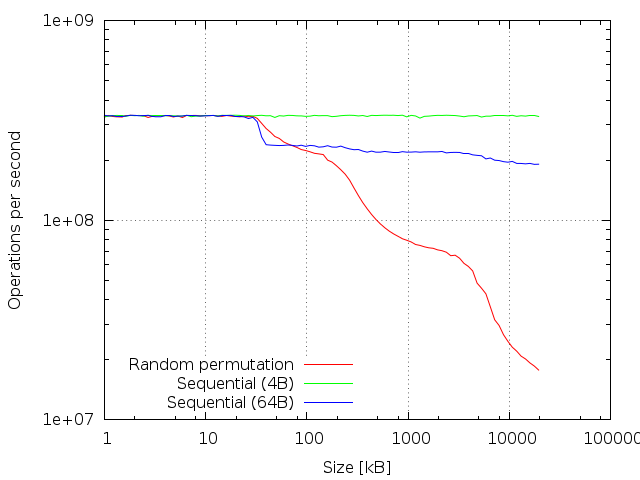
\includegraphics[scale=0.5]{results.png} 
\end{center}
\caption{Parallel Monte Carlo integration on Euler compute cluster.}
\label{fig1}
\end{figure}

\begin{figure}[ht]
\begin{center}
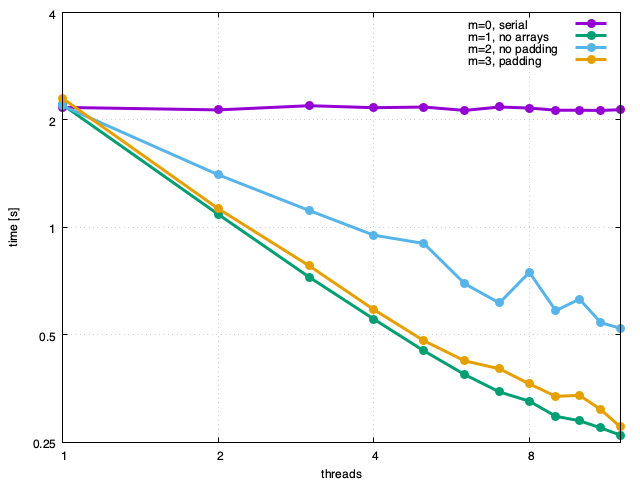
\includegraphics[scale=0.5]{results_mbp.png} 
\end{center}
\caption{Parallel Monte Carlo integration on 2018 Macbook Pro.}
\label{fig2}
\end{figure}

\subsection{Task c}
\begin{itemize}
    \item Yes, for the amount of tasks $N$ significantly larger than the number of threads, the workload is distributed evenly among the threads. For smaller $N$ this balance might not been exactly achievable.
    \item No, there is no perfect scaling as there is unparallelized overhead, but the modes \texttt{m=1} and \texttt{m=3} are not far off.
    \item A serial program and a single thread OpenMP program will get the same results provided the random generator seed remains unchanged. A multi-threaded OpenMP program on the other hand may show very small differences in the order of magnitude of machine precision when compared to the serial/single-thread results. This is due to the fact that each thread's random number generator is initialized with a different seed and also due to small numerical floating point rounding errors when adding the individual thread results.
\end{itemize}

\section{Question 2}

There is a problem with the global variable \texttt{pos} in the \texttt{if} statement starting on line 13: In order to write to the array \texttt{good\_members}, the value of \texttt{pos}
must be read in line 14. This read is not protected from race conditions with the atomic write on line 17. As \texttt{\#pragma omp atomic} cannot be extended to several statements, a possible (but still ugly)
solution would be to replace the \texttt{for} loop block from lines 12 to 19 with snippet~\ref{lst1}.

\begin{lstlisting}[float, caption={Proposed modification for correctness in task 2.}, label={lst1}]
    #pragma omp parallel for
    for (int i= 0; i < N; i++)
    {
        if (is_good(i)) // No change until here
        {
            int thread_pos{0}; // Define thread specific position variable
            #pragma omp critical // This block replaces the #pragma omp atomic section
            {
                thread_pos= pos; // Protected read
                pos++; // Protected write
            }
            good_members[thread_pos]= i; // Use thread specific variable
        }
    }
\end{lstlisting}


%\begin{thebibliography}{99}
%
%\bibitem{nasa}
%	NASA,
%	\emph{Haswell Processors},
%	online (\url{https://www.nas.nasa.gov/hecc/support/kb/haswell-processors_492.html}),
%	accessed 30-Sep-2018.
%
%\bibitem{intel}
%	Intel Corporation,
%	\emph{Intel Xeon Processor E5-2680 v3 Product Specifications},
%	online (\url{https://ark.intel.com/products/81908/}),
%	accessed 30-Sep-2018.
%	
%\bibitem{euler}
%	ETH Zurich,
%	\emph{scientific computing wiki: Euler},
%	online (\url{https://scicomp.ethz.ch/wiki/Euler#Euler_II}),
%	accessed 30-Sep-2018.	
%
%\bibitem{kou}
%	Petros Koumoutsakos,
%	\emph{HPCSE I Lecture Notes},
%	online (\url{http://www.cse-lab.ethz.ch/wp-content/uploads/2018/09/HPCSE_I_1_Intro.pdf}),
%	accessed 30-Sep-2018.
%
%\end{thebibliography}
%

%\appendix
%\section{Question 4, task d)}\label{app}
%\lstinputlisting{ex01_q4_task_d.cpp}
\end{document}